\documentclass[9pt,twocolumn,twoside]{../../styles/osajnl}
\usepackage{fancyvrb}
\journal{i524} 

\title{Using Hadoop and Spark for Big Data Analytics: Predicting Readmission of Diabetic patients}

\author[1,*]{Kumar Satyam}
\author[1,**]{Piyush Shinde}
\author[1,***]{Srikanth Ramanam}

\affil[1]{School of Informatics and Computing, Bloomington, IN 47408, U.S.A.}

\affil[*]{Corresponding authors: ksatyam@indiana.edu}
\affil[**]{Corresponding authors: pshinde@iu.edu}
\affil[***]{Corresponding authors: srikrama@iu.edu}

\dates{project-000, \today}

\ociscodes{Hadoop, Spark, MLlib, Ansible, Cloudmesh Client, Predictive Analysis}

% replace this with your url in github/gitlab
\doi{\url{https://github.com/cloudmesh/classes/blob/master/project/S17-IR-P004/report/report.pdf}}


\begin{abstract}
This project proposes and demonstrates the use of Hadoop and Spark on cloud to run predictive analytics using machine learning on large amount of data. Our case study is to predict the readmission likelihood for diabetes patients using their available medical history.
\newline
\end{abstract}

\setboolean{displaycopyright}{true}

\begin{document}

\maketitle

\tableofcontents % Print the contents section

\section{Introduction}
The idea behind this project is to introduce Hadoop/Spark over cloud infrastructure as a scalable and faster solution for predictive analysis using machine learning.

We chose the case study of predicting the likelihood of a diabetes patient getting readmitted within 30 days from the date of discharge using his/her available medical data. We approached this problem as a classification problem to classify the patients into  ‘Yes’ or ‘No’  classes, indicating whether the patient is likely to be readmitted or not in the next 30 days. We used different machine learning algorithms on the available data, after some pre-processing, to predict the same. The accuracy percentages obtained for all the utilized classification algorithms are included in the report. We also compared the results of Spark's Mllib algorithms against scikit-learn's algorithms and found that both yielded similar results.	

\begin{figure*}[h]\centering
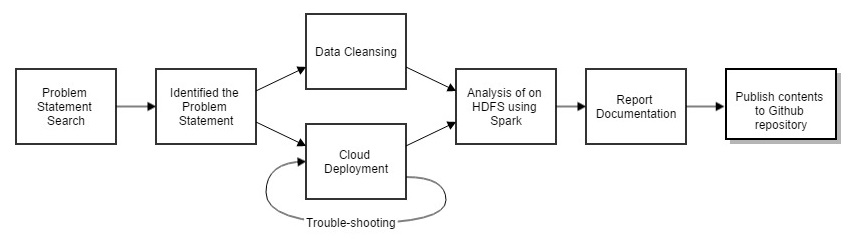
\includegraphics[width=\linewidth]{images/Workflow}
\caption{Workflow of the project}
\label{fig:workflow}
\end{figure*}

We approached the solution from a pure data perspective to address the challenge of lacking medical domain knowledge. For some basic information, we relied on the dataset description on UCI website \cite{www-dataset}, ICD-9 \cite{www-icd9} and earlier studies \cite{article-hindawi}. We followed a workflow as shown in figure \ref{fig:workflow}. 

Our other important goal is to propose an end-to-end solution that is scalable and faster. While our dataset is about 100,000 records, anticipating real-world scenarios with huge amounts of data we are proposing a Hadoop based solution. We are utilizing Spark for its faster processing \cite{www-sparkfast} and  advanced analytics through packages like Mllib \cite{www-mllib} which provides several commonly used machine learning algorithms. Finally we are implementing this solution over cloud infrastructure to meet our infrastructure requirements. This helped us demonstrate an end-to-end solution closer to real-world scenarios, where enterprises utilize cloud infrastructure in a pay per-use model. This helped us save time and resources in setting up the infrastructure.

We deployed our solution on two different clouds and obtained metrics to assess the infrastructure performance with our solution.  We also deployed our solutions on a distributed Hadoop/Spark environment built on on-premise machines. We compared the performance metrics of all the three infrastructure choices, with respect to our solution  and included them in this report.

\section{Architecture}

\begin{figure}[h]
\centering
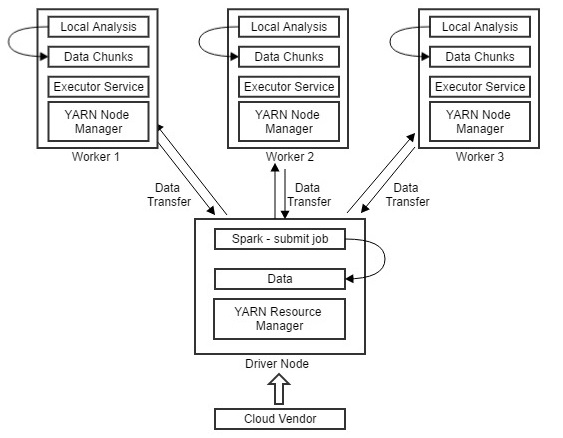
\includegraphics[width=\linewidth]{images/Architecture_Diagram}
\caption{Architecture Diagram}
\label{fig:arch}
\end{figure}

Figure \ref{fig:arch} gives an overview of our solution’s architecture. We deployed a spark driver node and three worker nodes. A driver node is a node that runs the driver program. It declares the transformations and actions on RDDs (Resilient Distributed Datasets) of data and submits such requests to the master \cite{www-rdd}. In practical terms, the driver is the program that creates the Spark Context \cite{www-sparkcontext}, connecting to a given Spark Master. It is a node where the yarn resource manager resides. A worker node is a node, which executes the program that involves individual data analysis task.
Running the spark-submit script from the master node starts the spark job. It divides the data into data chunks and transfers them to individual worker nodes. Then a processing task is performed on the data chunks on the individual worker nodes. The processed data and analytics results are then written back to the HDFS file system as needed.

We then deployed Hadoop and Spark on these machines to setup a HDFS Spark cluster on our cloud and on-premise machines. We stored our dataset on the Hadoop’s HDFS file system. Finally, we ran our predictive analytics application, which utilizes Mllib, on Spark cluster by launching it using spark-submit.

\section{Technologies}
\begin{table}[h!]
\centering
 \begin{tabular}[width=\linewidth]{|l l|}
 \hline
 \textit{Technology} & \textit{Usage}  \\  \hline
 \hline 
 \textbf{Hadoop}\cite{www-hadoop}/\textbf{Spark} \cite{www-spark} & Big Data Technologies  \\
 \hline
 \textbf{Python}\cite{www-python} & Development \\
  \hline
 \textbf{MLlib}\cite{www-mllib}/\textbf{scikit-learn}\cite{www-sklearn} & Machine Learning Library \\
 \hline
 \textbf{GitHub}\cite{www-github} & Project Repository \\
 \hline
 \textbf{Ansible}\cite{www-ansible} & Application Deployment \\ & $\&$ Configuration Management \\
 \hline
 \textbf{Chameleon}\cite{www-chameleon}, \textbf{JetStream}\cite{www-jetstream}, & Benchmarking \\
 \textbf{VirtualBox}\cite{www-vm} &\\
 \hline
 \textbf{LaTex} \cite{www-latex} & Document Preparation \\
 \hline
\end{tabular}
\caption{List of technologies used}
\label{table:techlist}
\end{table}

We used specific technologies for specific tasks in this project as listed in table \ref{table:techlist}:
\begin{itemize}
 \item \textbf{Hadoop}: Apache Hadoop is a framework for processing and storing huge amounts of data, commonly known as 'Big Data', in a distributed applications. It allows users to build scalable and highly available data applications. Hadoop has four modules: HDFS, YARN, MapReduce and Hadoop Common. Hadoop Distributed File System (HDFS) allows users to store large amounts of data.  YARN is the framework for job scheduling and resource management. MapReduce supports parallel processing of large data sets stored in the distributed environment through HDFS. Hadoop Common provides utilities that support other Hadoop modules.
 
 \item \textbf{Spark}: Spark runs on Hadoop and provides faster data processing capabilities for data on HDFS. It primarily uses a new data structure called Resilient Distributed Dataset (RDD) for processing. RDD is a read only multiset of data items distributed over cluster of virtual machines. Spark also has a new feature of fault tolerance and in the event of a primary master node failure, the secondary master takes over. Spark, unlike Hadoop applications, allows the iterative reading and writing in-memory. After processing it writes the data to HDFS.
 
 \item \textbf{Python}: We chose python as per our programming language. Python is one of the programming languages supported by Spark API through pyspark. We used it because of its simple syntax and data manipulation capabilities.
 \item scikit-learn: It is an open source Python library that provides Machine Learning algorithms and other utilities to preprocess and visualize data \cite{www-sklearn}.
 
 \item \textbf{MLlib}: Spark MLlib is the Spark’s machine learning library provides machine learning algorithms that can be applied on Resilient Distributed Datasets \cite{www-mllibguide}. It also provides other data manipulation utilities. MLlib has API available in Java, Python, Scala and R \cite{www-mllib}.
 
 
 
 \item \textbf{GitHub}: GitHub is 'a web-based Git or version control repository and Internet hosting service' \cite{www-wikigit}. We used Github repositories to store all the files related to documentation, ansible scripts and python code.
 \item \textbf{Ansible}: We are using ansible for automating deployment of our software on cloud. We used ansible scripts to automate deployment of cloudmesh client along with its pre-requisites like pip, virtualenv etc. We also used ansible for automating deployment of Hadoop and Spark.
\end{itemize}


\section{Cloud Infrastructure}
We have setup the required infrastructure by provisioning virtual machines on two cloud vendors, Chameleon, Jetstream and our on-premise machines.
\subsection{Chameleon Cloud}
Chameleon  is a collaborative cloud service primarily meant for research community. It allows users to explore problems ranging from the creation of Software as a Service to kernel support for virtualization. It is a good example of IAAS loaded with software defined networking and optimized virtualization technologies. We created three virtual machines on this cloud. One for Master node and two for worker nodes of Spark.

\subsection{Jetstream Cloud}
Jetstream is a cloud service which aims to provide researchers Jetstream’s development was led by Indiana University’s Pervasive Technology Institute (PTI) in collaboration with other universities \cite{www-jetstream} across the United States. This cloud service was used to provision the necessary virtual machines. We created three virtual machines on Jetstream for Spark cluster nodes.

\subsection{Virtual Box}
It is a fully virtualized hypervisor which gives the ability to spawn virtual machines in local commodity hardware. In fully virtualized environment, the guest OS  is not aware of the underlying  resources on which it is running as the hypervisor creates a complete simulation of the underlying hardware. 

A brief comparison of multiple attributes of the clouds used are displayed in table \ref{table:clouds}.

\begin{table}[h!]
\centering
 \begin{tabular}{|c|c c c|} 
 \hline
 \textit{Clouds} & \textit{Chameleon} & \textit{Jetstream} & \textit{VirtualBox}  \\ 
 \hline
 \hline 
 \textit{CPU} & Intel Xeon & Dual Intel & Intel Core  \\ 
 & X5550 & E-2680v3 "Haswell" & i5-6200U\\
 \hline 
 \textit{RAM} & 4 GB & 2 GB & 2 GB \\ 
\hline 
\textit{Number of CPU's} & 1 & 1 & 1 \\
\hline 
\textit{CPU Cores} & 1 & 1 & 2\\
\hline 
\textit{CPU Speed} & 2.3 GHz & 2.3 GHz & 2.3 GHz\\
\hline 
\end{tabular}
\caption{Comparison of cloud vendors}
\label{table:clouds}
\end{table}

\section{Automated Cloud Deployment: Ansible}
For this project, we used Ansible to automate the deployment of spark and its prequisites. The Ansible script is written such that we can leverage the cloudmesh client technology to deploy the spark cluster. The steps involved in the script can be seen in figure \ref{fig:ansible}.

\begin{figure}[h]
\centering
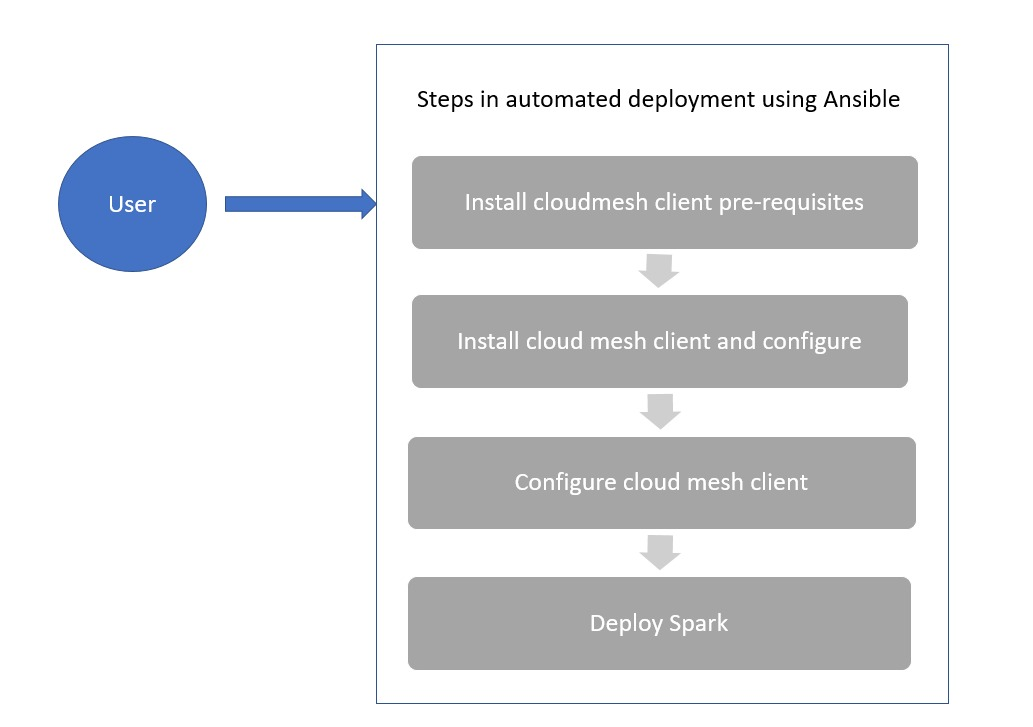
\includegraphics[scale = 0.28]{images/auto_deploy}
\caption{Automated Cloud Deployment using Ansible}
\label{fig:ansible}
\end{figure}


The Ansible playbook package constitutes 4 files.
\begin{enumerate}
\item \textit{ansible.cfg}: This file consists of configuration information.
\item \textit{playbook-cloudmesh-first-time-install.yml}: This file was used for deployment of cloudmesh client.
\item \textit{host}: This file contains the list of hosts.
\item \textit{hadoop-spark-playbook.yml}: This consists of the ansible code for redeployment of all the pre-requisites packages for cloudmesh client. This also deployment of spark using cloudmesh client.
\end{enumerate}

The following procedure has to be followed to run the Ansible script:
\begin{enumerate}
\item Install cloudmesh client for the first run 'playbookcloudmesh-first-time-install.yml' with the following command. This automates the deployment of cloudmesh client, which is a pre-requiste for installing Spark over our cloud infrastructure.  
\begin{verbatim}
ansible-playbook
playbook-cloudmesh-first-time-install.yml 
--ask-sudo-pass -vvvv
\end{verbatim}
 \item Open, $~$/.cloudmesh/cloudmesh.yaml and edit the following section,the entry with $< >$ should be customized as per your credentials.
\begin{verbatim}
profile:
     firstname: <first name>
     lastname: <last name>
     email: <email id>
     user: <chameleon/jetsream/other cloud username>
\end{verbatim}
\item Change the entry of active cloud to use your preferred cloud.  Example with chameleon is present below:
\begin{verbatim}
    active:
      - chameleon
    clouds:
      ...
\end{verbatim}
\item Under a cloud(chameleon/jetstream/..) change the following entry, the entry with <> should be customized as per your credentials:
\begin{verbatim}
credentials:
OS_PASSWORD: <enter your chameleon cloud password
here>
OS_TENANT_NAME: CH-818664
OS_TENANT_ID: CH-818664
OS_PROJECT_NAME: CH-818664
OS_USERNAME: <username>
\end{verbatim}
\item Also change, the type of OS and flavor you want for hadoop/spark cluster provided by your preferred cloud:
\begin{verbatim}
default:
        flavor: m1.medium
        image: CC-Ubuntu14.04
\end{verbatim}
\item Edit the file hadoop-spark-playbook.yml  in the section:
 'name:Preparing cloudmesh- setting default user', the entry with <> should be customized as per user credentials:
\begin{verbatim}
- name: Preparing cloudmesh- setting default user
become_user: "{{ lookup('env','USER') }}"
shell: cm default user=<chameleon/jetstream user>
\end{verbatim}
\item Now run the following command to deploy hadoop/spark cluster which will run the hadoop-spark-playbook.yml. It will again upgrade cloudmesh client, so it is up to date:
\begin{verbatim}
ansible-playbook hadoop-spark-playbook.yml
--ask-sudo-pass -vvvv
\end{verbatim}
\end{enumerate}

\section{Data Cleansing and Pre-processing}
The initial data set is publicly available on the UCI Machine Learning Repository \cite{www-dataset}.
The initial data set has information extracted from the database satisfying the following criteria \cite{article-hindawi}:
\begin{enumerate}
    \item Each row corresponds to an inpatient encounter (a hospital admission).
    \item All of the encounters are "diabetic" encounters, that is, one during which any kind of diabetes was entered to the system as a diagnosis.
    \item Each encounter also corresponds to a patient stay between 1 and 14 days.
    \item Laboratory tests were performed during the encounter.
    \item Medications were administered during the encounter.
\end{enumerate}

101,766 encounters were present in  the data set that satisfy the above five inclusion criteria. Each encounter consists of 55 features describing the diabetic encounters, including demographics, diagnoses, diabetic medications, number of visits in the year preceding the encounter, and payer information. We defined the readmission  field with 2 values: “YES,” for cases where the patient was readmitted within 30 days of discharge and “NO,” for both readmission after 30 days scenario and no readmission at all.

Diagnosis 1, 2 and 3 had many categorical values in the form of ICD-9 codes and had missing values. These ICD-9 codes were sorted and grouped into 9 categories, namely Circulatory, Respiratory, Digestive, Diabetes, Injury, Musculoskeletal, Genitourinary, Neoplasms and Other based on the ICD-9 codes \cite{article-hindawi}. The missing values were assigned the group ‘Other’.

This data set had several  features with empty fields. So we removed the features missing high percentages of data as they affect our analysis. The removed  features were weight, medical specialty and payer code. The race attribute had 2$\%$ missing values which were filled by the mode value ‘Caucasian’.

Observations only with unique patient ids were considered, excluding those with discharge disposition corresponding to the patient’s death.

We filtered our data set according to the above-mentioned constraints and retained  62,937 encounters each corresponding to an unique patient and 55 features describing such encounter. We prepared three data-sets to test the multiple machine learning algorithms (Stochastic Gradient Descent, Gaussian Naïve Bayes, K-means and Decision Tree).  Finally we also removed the patient id and encounter id  as they were not relevant to learning algorithms.

We used one hot encoding to convert the categorical data features  to numerical data. This creates new dummy features to represent the categorical data in numerical format.

The first data set was prepared using one hot encoding on the original data (with 62,937 observations), that resulted in 136 features representing the original 55 features.

For our second data set we implemented feature selection using a Variance Threshold algorithm that removes all low-variance features \cite{www-vt}. We set a variance threshold of '0.8'.

The data set B was formed using this algorithm, which helped extract 26 features.

The original data contains the age attribute grouped in 10-year intervals from 0 to 100 years. For the third data set we grouped the 10 intervals to 3 intervals by combining the age groups younger than 30, 30-60 and older than 60 years. One-hot encoding was then applied to form the third data set. This data set contained 129 features.



\section{Preliminary Data Analysis}
The unit of our analysis is an encounter; to keep the observations independent, we only analyzed one encounter per patient.
We performed early data analysis in python in a local machine. We implemented four classification algorithms using scikit-learn library on each of the 3 data sets created. The data sets were first divided in training and testing set. The training set had about 80$\%$ observations (5000 observations approx.) whereas the testing set had the remaining 20$\%$ observations (12937 observations). Each of the algorithms provided by scikit-learn were used following in the manner:
\begin{enumerate}
\item Create and fit a model using the observations and readmission of the training set.
\item Predict labels of the testing set.
\item Calculate the accuracy using the predicted labels and true labels of the testing set. The parameters needed in implementing the above-mentioned algorithms were set so as to be valid to our data, give optimum results and make the results to be reproducible.
\end{enumerate}
KMeans clustering gave us approximately 55$\%$ accuracy with all the three data sets.  Though it is an unsupervised learning algorithm, we used it to examine if the clustering divided the data into readmission classes, Yes and No, to an acceptable level. We concluded that clustering based on the Euclidean distance may not be the right approach for this classifying this data set. The accuracy percentages obtained  for other classification algorithms can be found  in the Table \ref{table:sklearn}.

\begin{table}[h!]
\centering
 \begin{tabular}{|c c c|} 
 \hline
 \textit{Classification Technique} & \textit{Number of Features} & \textit{Accuracy ($\%$)}\\ 
 \hline
 \hline 
  SGDClassifier & 136 & 90.68 \\  & 26 & 86.31\\
  & 129 & 86.96\\
 \hline 
  GaussianNB & 136 & 10.43 \\  & 26 & 88.30\\
  & 129 & 9.96\\ 
 \hline 
   KMeans & 136 & 55.26 \\ 
   & 26 & 55.24\\
  & 129 & 55.26\\ 
 \hline 
DecisionTreeClassifier & 136 & 83.35 \\ & 26 & 82.50\\
  & 129 & 83.28\\
\hline 
\end{tabular}
\caption{Results from scikit-learn}
\label{table:sklearn}
\end{table}



\section{Data Analysis on Spark cluster}
We performed data analysis on Spark cluster using pyspark MLlib on data stored on HDFS.

\subsection{Start the Spark service}

Start the service of spark using the following command:
\begin{verbatim}
$SPARK_HOME/sbin/start-all.sh
\end{verbatim}



Stop the service of spark using the following command:
\begin{verbatim}
$SPARK_HOME/sbin/stop-all.sh
\end{verbatim}


Using the command 'jps' we get a list of the following services:
\begin{verbatim}
 nodemanger
 resourcemanger
 master
 namenode
 applicationmaster
\end{verbatim}


\subsection{Data Storage}
 Uploading input data and code to Driver Node After the Spark setup is ready for the deployment, the data is pushed from the localhost to the remote spark master node. For this we used an ansible script.
\begin{enumerate}
 \item Ansible script
\begin{enumerate}
 \item In the host files we set the target master(driver node) IP address as follows:
 \begin{verbatim}
[remotehosts]
129.114.33.106 ansible_ssh_user=cc
\end{verbatim}
\item  Now , add the following entry in the yaml file to transfer the file to destination
\begin{verbatim}
- hosts: remotehosts
   tasks:
     - name: Transfer file from local to
     satyam-001
       synchronize:
         src: /home/<username>/ansible
         script/ansible-spark/traindat.csv
         dest: /home/cc/
         mode: push
       delegate_to: 127.0.0.1
\end{verbatim}
\end{enumerate}
\item Using Github we uploaded the input data csv file and python execution code to a git repository. We installed git package in the spark driver node. We used ‘wget’ command  with the repository path to download  the data set to the virtual machine.
\end{enumerate}

 
After the data is downloaded to the virtual cloud machine, we uploaded the file to HDFS through the following command.
\begin{verbatim}
Hdfs dfs  –put  <source file path>  <hdfs-folderpath>
\end{verbatim}

This HDFS file serves as an input for our analytics application.

\subsection{Launching Data Analysis Application}
 We used  python programming language to develop an application that  performs predictive analytics tasks. We leveraged  pyspark.mllib library for machine learning algorithms.
 
We launched our application code using the following command
\begin{verbatim}
$ ./bin/spark-submit --class path.to.your.Class 
--master yarn --deploy-mode cluster [options] 
<app jar> [app options]
\end{verbatim}

 There are 4 main steps to each implementation of.
 \begin{itemize}
  \item Input formatting: MLlib classes expect RDD’s of LabeledPoints. For this we parsed the data and converted each entry into a LabeledPoint , with label specifying the true output class.
\item Next, the processed data frame is divided into train and test datasets.
\item Train the model with the algorithm and training data
\item After  training, We used the model to predict the classes for test data and calculate the accuracy
 \end{itemize}

\section{Results}

\begin{table}[h!]
\centering
 \begin{tabular}{|c c c|} 
 \hline
 \textit{Classification Technique} & \textit{Number of Features} & \textit{Accuracy ($\%$)}\\ 
 \hline
 \hline 
  SGDClassifier & 136 & 90.88
 \\  & 26 & 90.99\\
  & 129 & 90.88\\
 \hline 
  GaussianNB & 136 & 84.97
 \\  & 26 & 85.02\\
  & 129 & 84.987
\\ 
 \hline 
   KMeans & 136 & 55
 \\ 
   & 26 & 55\\
  & 129 & 55\\ 
 \hline 
DecisionTreeClassifier & 136 & 91.01 \\ & 26 & 90.75\\
  & 129 & 90\\
\hline 
\end{tabular}
\caption{Results from Spark MLlib}
\label{table:mllib}
\end{table}

Kmeans did not successfully separate the data class wise as observed in scikit-learn library, as shown in table \ref{table:mllib}.  We used  supervised classification algorithms namely decision tree, logistic stochastic gradient descent and naïve bayes. We obtained good accuracies of 80-90$\%$ with classification algorithms.

These can be found in the below table.
Similar analysis in a real world scenario can be utilized to predict the readmission likelihood using medical records of diabetes patients. This enables doctors to  pay special attention to those patients, identify the causal factors and give preventive care.



\section{Benchmarking}

In the figure \ref{fig:bench} we are displaying the time taken to run each of the four algorithms in different clouds. The four algorithms are SGD Classifier, Gaussian Naïve Bayes, kmeans and Decision Tree Classifier.

\begin{enumerate}
 \item The complexity of the algorithm. For example,  kmeans clustering has  O(n log n) time complexity which is worse than Gaussian Naïve Bayes and hence takes more time.
 \item The compute resources used.  For example the chameleon cloud takes less time to execute any other algorithm because the RAM configuration for the VMs of chameleon cloud is better than any other VMs.
 \item The network latency between the hosts: The VMs which are provisioned on clouds can be on different hosts spread across different racks of datacenters and even datacenters across geographies. This may result in network latency and affect the runtime of a program running in a distributed environment.
\end{enumerate}

\subsection{Computation time of algorithms in clouds}
Figure \ref{fig:bench} shows the performance of multiple machine learning algorithms using Spark MLlib in multiple clouds.
\begin{figure}[h]
\centering
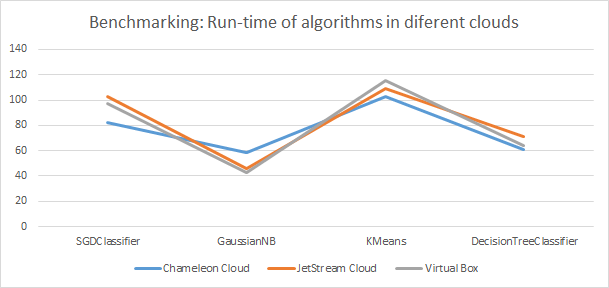
\includegraphics[scale=0.85]{images/Benchmarking}
\caption{Run-time in different clouds.}
\label{fig:bench}
\end{figure}

\subsection{Comparison of multiple algorithms in Spark MLlib vs scikit-learn}

We can see from figure \ref{fig:accmllib} that accuracies between multiple algorithms in MLlib are almost smiliar. 

\begin{figure}[h]
\centering
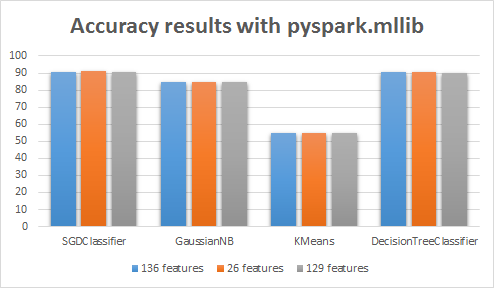
\includegraphics[width=\linewidth,scale=1]{images/accmllib}
\caption{Accuracy Results with pyspark.mllib}
\label{fig:accmllib}
\end{figure}

Figure \ref{fig:mllibvssklearn} shows accuracy results of multiple machine learning algorithms in scikit-learn vs MLlib.

\begin{figure}[h]
\centering
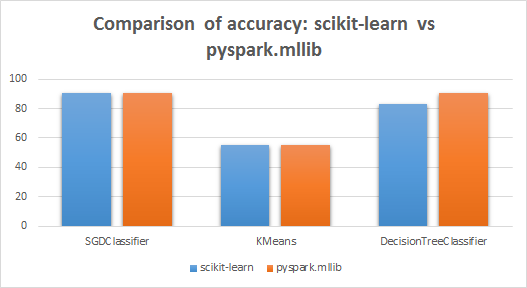
\includegraphics[width=\linewidth,scale=1]{images/mllibvssklearn}
\caption{Accuracy Results: scikit-learn vs pyspark.mllib}
\label{fig:mllibvssklearn}
\end{figure}

\section{Troubleshooting}
We encountered several errors while running different commands in the Linux terminal. We have listed some of the commands and errors encountered while executing them followed by the steps to resolve them.
\begin{enumerate}
 \item \textbf{Command}: cm ssh key upload
 
 \textbf{Error 1}: Permission denied (public key)
 
 \textbf{Error 2}: Problem uploading key <username> to cloud chameleon:
 The request you have made requires authentication
 
 \textbf{Resolution}: \\
 cm ssh-key delete <username>-001\\
 cm ssh-key delete <username>-001 cloud = chameleon\\
 cm ssh-key add\\
 cm ssh-key upload\\
 cm key refresh
 
 \item \textbf{Command}: cm hadoop deploy
 
 \textbf{Error}: IndexError: list index out of range

 \textbf{Resolution}: Use the following image:
 
cm cluster define --count 3 --image CC-Ubuntu14.04

\item \textbf{Command}: cm hadoop deploy

 \textbf{Error}: INFO: Waiting for cluster to be accessible
DEBUG: Running cmd: ansible all -m ping -u ubuntu
stack-0011 | UNREACHABLE! => $\{$
"changed": false, 
"msg": "SSH encountered an unknown error during the 
connection. We recommend you re-run the command using 
-vvvv, which will enable SSH debugging output to help 
diagnose the issue", 
"unreachable": true
$\}$

\textbf{Resolution}: Use the following image:

cm cluster define --count 3 --image CC-Ubuntu14.04


 \item \textbf{Command}: cm hadoop sync
 
 \textbf{Error}: no github account associated
 
 \textbf{Resolution}: 
 
 git config --global user.name "username"
 git config --global user.email "emailid"
 

 \item \textbf{Command}: apt-get install git
 
 \textbf{Error}: Permission denied when running "apt-get install git" command
 
 \textbf{Resolution}: Exit from the current hadoop user using \textit{exit} command. The user will change to ‘cc’ that has the root privileges. Install  the package through the 'cc' user log-in back as the hadoop user to use the installed package .
\end{enumerate}

The "Cm refresh on" command can be used most of the times to resolve multiple errors.









    
    

\section{Conclusion}
We demonstrated the implementation of a big data based  predictive analytics solution using Hadoop, Spark and Spark’s MLlib machine learning algorithms. We predicted the readmission likelihood with an accuracy 90$\%$ by analyzing the data stored on HDFS.  While Hadoop provided us a distributed file system for storing large amounts of data, Spark provided us big data processing capabilities and several libraries to accomplish several common processing and analytics tasks. We used MLlib library’s algorithms to achieve similar results as obtained with scikit-learn library. These technologies can be used to build similar solutions for real world scenarios requiring processing and performing analytics over big data.  Similar applications can be built leveraging   Spark’s ability to process streams of data and support for machine learning algorithms. 

\section{Acknowledgments}
This project was a part of the Big Data Software and Projects (INFO-I524) course. We would like to thank Professor Gregor von Laszewski and the associate instructors for their help and support during the course. 

\bibliography{references}

\end{document}
